\section{Sketch-Guided Equality Saturation} %\todo{nice if this section starts on page 8}
\label{sketching}

This section introduces \emph{sketch-guided equality saturation}, a novel semi-automated process offering a trade-off between manually written rewriting strategies and fully automated equality saturation.
The programmer guides multiple equality saturations by specifying a sequence of sketches that describe how a program should evolve during optimization.
While rewriting strategies require fine-grained phase ordering, sketch-guided equality saturation enables coarse-grained phase ordering.
For example, instead of specifying how to sequence thousands of rewrite rules to achieve matrix multiplication blocking, specifying just two sketches suffices.

\subsection{The Intuition for Sketches}

When designing optimizations, programmers often visualize the desired \emph{shape} of the optimized program. An optimization, e.g.~with rewriting strategies or schedules, is often illustrated with program snippets that explain its effect \cite{koehler2021-elevate-imgproc, ragan2013-halide, chen2018-tvm, adams2019-learning, sioutas2020-schedule, ikarashi2021-guided, anderson2021-efficient}. Indeed, this is exactly how we have explained the loop nest blocking optimization in \cref{fig:mm-rewrite}.
% To convey the impact of the defined \Elevate{} strategies, the paper describes the program shape at different optimization stages.
%In~\cite{koehler2021-elevate-imgproc} these program snippets where added to the paper only to explain the effect of the complex rewrite sequences that were manually orchestrated by a programmer.

Our \emph{key new insight} is that explanatory program snippets can be formalized as sketches and used to guide an optimization search, instead of manually writing strategies or schedules that perform the optimization directly.
\emph{Sketches} are program patterns that capture intuitions about the program shape while leaving details unspecified.
The guided optimization search still performs rewriting with semantic preserving rules, allowing sketches to leave out details without sacrificing correctness.
We define sketches formally in \cref{sketch-def}.
% This sketch resembles the snippet in \cref{harris-shape3} but adds program holes (\inlineRiseSketch{?}) and constraints (\inlineRiseSketch{contains}) to explicitly elide program details.

\begin{figure}
\begin{minipage}{0.75\linewidth}
\begin{center}
\begin{rise-sketch}[caption={Sketch for the \goalStyle{baseline} matrix multiplication goal}, label={mm-baseline-sketch}]
containsMap(m,                | for m:
 containsMap(n,               |  for n:
  containsReduceSeq(k,        |   for k:
   containsAddMul)))          |     .. + .. * ..
\end{rise-sketch}
\begin{rise-sketch}[caption={Sketch for the \goalStyle{blocking} matrix multiplication goal}, label={mm-blocking-sketch}]
containsMap(m / 32,           | for m / 32:
 containsMap(n / 32,          |  for n / 32:
  containsReduceSeq(k / 4,    |   for k / 4:
   containsReduceSeq(4,       |    for 4:
    containsMap(32,           |     for 32:
     containsMap(32,          |      for 32:
      containsAddMul))))))    |        .. + .. * ..
\end{rise-sketch}
\begin{rise-sketch}[caption={Sketch guide specifying how to split loops for \goalStyle{blocking}}, label={mm-blocking-split-sketch}]
containsMap(m / 32,           | for m / 32:
 containsMap(32,              |  for 32:
  containsMap(n / 32,         |   for n / 32:
   containsMap(32,            |    for 32:
    containsReduceSeq(k / 4,  |     for k / 4:
     containsReduceSeq(4,     |      for 4:
      containsAddMul))))))    |        .. + .. * ..
\end{rise-sketch}
\end{center}
\end{minipage}
\end{figure}

We illustrate by presenting the sketches for matrix multiplication blocking.
\Cref{mm-baseline-sketch} shows the sketch for the unoptimized \goalStyle{baseline} goal, specifying the desired program structure as two nested \inlineRise{map} patterns and a nested \inlineRise{reduce}, with innermost addition and multiplication operations. The formal definitions of \inlineRiseSketch{containsMap}, \inlineRiseSketch{containsReduceSeq} and \inlineRiseSketch{containsAddMul} are in \cref{sketch-def}.
The comments on the right show the equivalent nested \inlineRise{for} loops, using the same intuition as in \cref{fig:mm-rewrite}.

The sketch describing the \goalStyle{blocking} goal in \cref{mm-blocking-sketch} corresponds to the optimized program where the "loop nests" have been split and reordered so that the iteration space is chunked into blocks of $4 \times 32 \times 32$, each processed by the three innermost \inlineRise{for} loops.

Searching for the \goalStyle{blocking} goal can be made more tractable by specifying intermediate \emph{sketch guides}, and \cref{mm-blocking-split-sketch} is an example.
This sketch guide describes a program shape where the \inlineRise{map} and \inlineRise{reduce} patterns have been split but not yet reordered.

\Elevate{} rewriting strategies, as seen before in \cref{lst:elevate-blocking}, are detailed \emph{imperative} specifications of how to rewrite the program. In contrast, a sketch is a \emph{declarative} specification of the optimization goal, and equality saturation is used to search for a sequence of rewrites to achieve that goal.
A sequence of sketches (e.g., \cref{mm-blocking-split-sketch} followed by \cref{mm-blocking-sketch}) may be used to achieve a desired optimization when the equality saturation search with a single sketch as a goal does not succeed.

%In contrast to the \Elevate{} rewriting strategy shown in \cref{lst:elevate-blocking}, sketches focus on the effect the optimization has on the program, rather than how the transformation is performed step-by-step.



% Instead of specifying a detailed rewrite order through \Elevate{} strategies, sketch-guided equality saturation enables programmers to declaratively specify their desired optimization goal via sketches.

\subsection{Sketch Definition}
\label{sketch-def}

% A sketch represents a set of terms in a declarative way and is used to specify a rewriting goal without having to write down an entire program.
% It allows to be succinct by omitting many details, and to let equality saturation figure out these details.
% A sketch can be more or less precise by restricting $R(s)$ more or less compared to $T$.
% \todo{are sketches new? no; but previously published definition is different.. cite and explain difference? use different name?}

\newcommand{\sLang}{\textsc{SketchBasic}}

Sketches are specified in a  \sLang{} language with just four constructors.
The  syntax of \sLang{} and the set of terms that the constructors represent are defined in \cref{fig:sketch-lang-rep}.
A sketch $s$ represents a set of terms $R(s)$, such that $R(s) \subset T$ where $T$ denotes all terms in the language we rewrite.
We say that any $t \in R(s)$ satisfies sketch $s$.

The $?$ sketch is the least precise, representing all terms in the language.
The $F(s_1, .., s_n)$ sketch represents all terms that match a specific $n$-ary function symbol $F$ from the term language, and whose $n$ children satisfy sketches $s_i$.
The $contains(s)$ sketch represents all terms containing a term that satisfies sketch $s$.
Finally, the $s_1 \lor s_2$ sketch represents terms satisfying either $s_1$ or $s_2$.

\begin{figure}
  \begin{lstlisting}[mathescape, basicstyle={\linespread{.75}\ttfamily\normalsize}, frame=none, xleftmargin=0.25\linewidth]
  $S$ ::= $?$ | $F(S, .., S)$ | $contains(S)$ | $S \lor S$
  \end{lstlisting}
%   \caption{Grammar of \sLang{}.}
%   \label{fig:sketch-lang}
% \end{figure}
% \begin{figure}
    \begin{align*}
      R(?) &= T = \{ F(t_1, .., t_n) \} \\
      R(F(s_1, .., s_n)) &= \{ F(t_1, .., t_n) \mid t_i \in R(s_i) \} \\
      R(contains(s)) &= R(s) \cup \{ F(t_1, .., t_n) \mid \exists t_i \in R(contains(s)) \} \\
      R(s_1 \lor s_2) &= R(s_1) \cup R(s_2)\\[-2em]
    \end{align*}
    \caption{Grammar of \sLang{} (top) and terms represented by \sLang{} (bottom).}
    \label{fig:sketch-lang-rep}
\end{figure}

When rewriting terms in a typed language, sketches may be annotated with a type sketch ($s :: pt$) constraining the type of terms.
If $R(pt)$ denotes the set of terms satisfying the type sketch $pt$, then $R(s :: pt) = R(s) \cap R(pt)$.
The grammar of type sketches depends on the language we rewrite.
We elide type sketches from our definition of \sLang{} for simplicity, but use them for \Rise{}.

Writing a useful sketch to guide an optimization search requires striking a balance between being too precise and too vague.
An overly precise sketch may exclude valid optimized programs with a slightly different structure.
An overly vague sketch may lead to finding undesirable programs.
This balance also interacts with the rewrite rules involved, since programs that may be found by the search are $R(s) \cap EQ(t, rules)$ where $EQ(t, rules)$ represents the set of terms that can be discovered to be equivalent to the initial term $t$ according to the given $rules$.
This means that using a more restricted set of rules generally enables specifying less precise sketches.
How to best select rules and write effective sketches are topics for future work.

\textit{Sketch Abstractions}.
Sketch abstractions are defined by combining generic constructs from \sLang{} with type annotations from the term language.
To illustrate, \cref{rise-sketch-abs} shows the sketch abstractions for our \Rise{} matrix multiplication case study.
%Sketch abstractions are defined for our matrix multiplication case study by combining generic constructs from \sLang{} with \Rise{}-specific type annotations (\cref{rise-sketch-abs}).
Here \inlineRise{$\to$} is a function type, and \inlineRise{n.dt} an array type of \inlineRise{n} elements of domain type \inlineRise{dt}.
The type annotations restrict the iteration domains of patterns like \inlineRise{map} and \inlineRise{reduceSeq}.
We use similar definitions for other language constructs.

% def containsMap(dt: DataTypePattern, f: sketch): sketch =
%   contains(app(map :: ?t ->: dt ->: ?t, f))
% def containsMap(n: NatPattern, f: sketch, in: sketch): sketch =
%   contains(app(app(map :: ?t ->: n.?dt ->: ?t, f), in))
% def containsMapPar(n: NatPattern, f: sketch): sketch =
%   contains(app(omp.mapPar :: ?t ->: n.?dt ->: ?t, f))
% def containsMapPar(dt: DataTypePattern, f: sketch): sketch =
%   contains(app(omp.mapPar :: ?t ->: dt ->: ?t, f))
% def containsMapPar(n: NatPattern, f: sketch, in: sketch): sketch =
%   contains(app(app(omp.mapPar :: ?t ->: (n.?dt) ->: ?t, f), in))

% def containsMapSeq(n: NatPattern, f: sketch): sketch =
%   contains(app(mapSeq :: `?t` ->: (n`.``?dt`) ->: `?t`, f))
\begin{figure}
\begin{minipage}{0.75\linewidth}
\begin{center}
\begin{rise-sketch}[label={rise-sketch-abs}, caption={Some sketch abstractions used in the paper.}]
def containsMap(n: NatSketch, f: Sketch): Sketch =
  contains(app(map :: ?t $\to$ n.?dt $\to$ ?t, f))
def containsReduceSeq(n: NatSketch, f: Sketch): Sketch =
  contains(app(reduceSeq :: ?t $\to$ ?t $\to$ n.?dt $\to$ ?t, f))
def containsAddMul: Sketch =
  contains(app(app($+$, ?), contains($\times$)))
\end{rise-sketch}
\end{center}
\end{minipage}
\end{figure}

\begin{figure}[b]
  \centering
  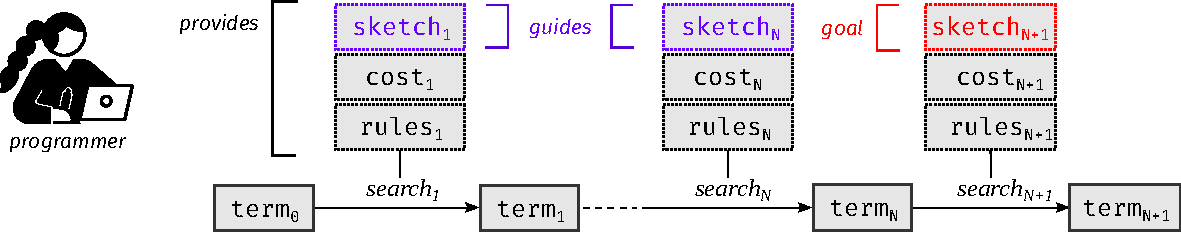
\includegraphics[width=0.9\linewidth]{media/sketch-guided-es.pdf}
  \caption{Sketch-Guided Equality Saturation.
  The programmer provides $N$ intermediate sketch guides and $1$ final goal sketch.
  Starting from the input term, $N+1$ consecutive equality saturation searches attempt to find a term satisfying each sketch, using the associated cost models and sets of rules (\cref{fig:search-diagram}).}
  \label{fig:sketching}
\end{figure}

\subsection{Sketch-Guided Equality Saturation}
\label{sketching-sub}

The process of guiding equality saturation with a sequence of sketches is illustrated in \cref{fig:sketching}.
The programmer provides a sequence of $N$ intermediate sketch guides and a final goal sketch: $sketch_1,\,..,\,sketch_{N+1}$.
Successive equality saturation searches are performed to find equivalent terms that satisfy each sketch in the sequence. As each sketch may be satisfied by many terms, the programmer must also provide a sequence of cost models $cost_1, .., cost_{N+1}$ to select the term to be used as the starting point for the next search. Sets of rewrite rules ($rules_1, .., rules_{N+1}$) are provided to grow the e-graph in each search. The cost model and set of rules may be identical for many or all of the searches, but we show examples in \cref{evaluation} where selectively restricting the set of rules reduces search runtime. \Cref{fig:search-diagram} shows how each search is performed, and how these searches differ from standard equality saturation.



\begin{figure}[b]
\begin{minipage}{0.52\linewidth}
\begin{center}
\begin{lstlisting}[numbers=left, xleftmargin=2em, label={fig:sketching-alg}, caption={Sketch-Guided Equality Saturation Algorithm}, escapechar=|, mathescape=true, morekeywords={def, if, then, else},captionpos=b,abovecaptionskip={.5\baselineskip},moredelim={*[is][\rmfamily\itshape\color{black!50}]{~}{~}}]
def SGES(term, params): Option[Term] = |\label{line:sges}|
 if params.isEmpty
 then Some(term)
 else search(term, params.head) |\label{line:sges-search}|
      .and_then($\lambda$t. SGES(t, params.tail)) |\label{line:sges-rec}|
   
def search(term, param): Option[Term] =
 (sketch, cost, rules) = param
 g = ~create empty e-graph~
 normTerm = normalize(term) |\label{line:normalize}|
  ~using a configurable normal form~
 e = g.add(normTerm)
 ~grow~ g ~using~ rules ~until~ found(g, e, sketch) 
 if found(g, e, sketch) then |\label{line:found}|
  Some(extract(g, e, sketch, cost)) |\label{line:beam-extraction}|
 else
  None
\end{lstlisting}
%\begin{lstlisting}[numbers=left, xleftmargin=2em, label={fig:sketching-alg}, caption={Sketch-Guided Equality Saturation Algorithm}, escapechar=|, morekeywords={def, if, then, else},captionpos=b,abovecaptionskip={.5\baselineskip},moredelim={*[is][\rmfamily\itshape\color{black!50}]{~}{~}}]
%def SGES(term, params): Option[Term] =
% if params.isEmpty
% then Some(term)
% else
%  (sketch, cost, rules) = params.head
%  g = ~create empty e-graph~
%  normTerm = normalize(term) |\label{line:normalize}|
%   ~using a configurable normal form~
%  e = g.add(normTerm)
%  ~grow~ g ~using~ rules ~until~ found(g, e, sketch) 
%  if found(g, e, sketch) then |\label{line:found}|
%   nextTerm = extract(g, e, sketch, cost) |\label{line:beam-extraction}|
%   SGES(nextTerm, params.tail)
%  else
%   None
%\end{lstlisting}
\end{center}
\end{minipage}\hfill%
\begin{minipage}{0.45\linewidth}
\begin{center}
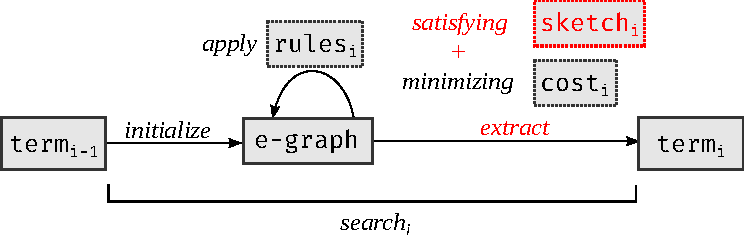
\includegraphics[width=\linewidth]{media/equality-saturation-sketches.pdf}
\captionof{figure}{Sketch-Satisfying Equality Saturation implementing each $search_i$.  Changes made to standard equality saturation are highlighted in red.}\label{fig:search-diagram}%
\end{center}
\end{minipage}
\end{figure}

The pseudo-code for the sketch-guided equality saturation algorithm is shown in \cref{fig:sketching-alg}.
The entry point is the \inlineRise{SGES} function (line \ref{line:sges}) that takes  a \inlineRise{term} and a sequence of sketches, cost models and rewrite rules (\inlineRise{params}). It repeatedly \inlineRise{search}es (line \ref{line:sges-search}) for each sketch using the associated cost model and rewrite rules, and outputs a term if found, otherwise nothing.

At the beginning of each \inlineRise{search}, we may normalize the input term (line \ref{line:normalize}) to apply destructive rewrites that are always desired before starting a purely additive equality saturation.
For our matrix multiplication running example we use $\beta\eta$ normal form.
The \inlineRise{extract} function (line \ref{line:beam-extraction}) is used to extract a term from the e-graph that satisfies the specified sketch while minimizing the specified cost model, and we describe it in the next subsection.
In this paper, we terminate equality saturation as soon as a program satisfying the current sketch is found, whether or not the cost could be further improved by a longer search.
This is because we give more value to satisfying the sketch than to minimizing the cost.
Other applications of sketch-guided equality saturation could use different stopping criteria.
The \inlineRise{found} function (line \ref{line:found}) is used to stop growing the e-graph by checking whether \inlineRise{extract} would succeed.

\subsection{Sketch-Satisfying Extraction}
\label{beam-extraction}

To \inlineRise{extract} the best program that satisfies a \sLang{} sketch $s$ from an e-graph $g$ we define a helper function $E(c, s, g)$, where $c$ is a cost function that must be monotonic and local.
%\todo{Do you think the cost in E(c, s, g) can be non-monotonic?
%Yes, but it would require designing a different extraction algorithm that solves a harder problem. For %example, if optimizing multiple objectives, one could extract a Pareto front for each e-class instead of a %single program. Alternatively, extraction could be modeled as an integer linear programming problem, as done %in other works.}
% , i.e., it must have the following signature:
% $$ c(F(k_1: K, .., k_n : K)): K.$$
While \inlineRise{extract} returns a program from an e-class $e$, the helper $E$ returns a map from e-classes to optional tuples of costs and terms.
After invoking $E$ we simply look up the e-class $e$ in the map and extract the term from the optional tuple.
For efficiency, we memoize previously computed results of $E$.
The \inlineRise{extract} function is recursively defined over the four \sLang{} cases as follows.

\smallskip

\textbf{Case 1:} $\bm{s =\ ?}$.
This case is equivalent to extracting the programs minimizing $c$ from the e-graph.
We implement this extraction as an e-class analysis (\cref{eqsat}) with data type $D = \text{Option}[(k, t)]$ and functions $make$ that constructs analysis data and $merge$ that combines analysis data from e-nodes in the same e-class:
\small
\begin{align*}
make(F(d_1, .., d_n)) = &\begin{cases}
  Some\left(\begin{array}{l}
    c(F(k_1, .., k_n)),\\
    F(t_1, .., t_n)
  \end{array}\right) & (k_i, t_i) \in d_i \\
  None & \text{otherwise}
\end{cases}\\
% \end{align*}
% \begin{align*}
merge(d_1, d_2) = &\begin{cases}
  \text{if } k_1 \leq k_2 \text{ then } d_1 \text{ else } d_2 & (k_i, \_) \in d_i \\
  d_1 & (k_1, \_) \in d_1 \\
  d_2 & (k_2, \_) \in d_2 \\
  None & \text{otherwise}
\end{cases}
\end{align*}
\normalsize

\textbf{Case 2:} $\bm{s = F(s_1, .., s_n)}$.
We consider each e-class $e$ containing $F(e_1, .., e_n)$ e-nodes and the terms that should be extracted for each child e-class $e_i$.
We write $E(c,s, g)[e]$ for indexing into the map returned by $E$:
\small
\begin{align*}
E(c, F(s_1, .., s_n), g)[e] = \begin{cases}
  Some(c(F(k_1, .., k_n)), F(t_1, .., t_n)) & (k_i, t_i) \in E(c, s_i, g)[e_i] \\
  None & \text{otherwise}
\end{cases}
\end{align*}
\normalsize

\textbf{Case 3:} $\bm{s = contains(s_2)}$.
We use another e-class analysis and initialize the analysis data to $E(c, s_2, g)$ corresponding to the base case where $R(s_2) \subset R(contains(s_2))$.
To $make$ the analysis data we consider all terms that would contain terms from $s_2$ and keep the best by folding them using $merge$:
\small
\begin{align*}
make(&F(d_1, .., d_n)) = foldl~merge~None \\
  \{ &Some(c(F(k_1, .., k_j, .., k_n)), F(t_1, .., t_j, .., t_n)) \mid
     \quad i \neq j, (k_i, t_i) \in E(c, ?, g)[e_i], (k_j, t_j) \in d_j \}
\end{align*}
\normalsize

To $merge$ the analysis data, we do the same as for $s =\ ?$.

\medskip

\textbf{Case 4:} $\bm{s = s_1 \lor s_2}$. We $merge$ the results from $s_1$ and $s_2$:
\small
$$ E(c, s_1 \lor s_2, g)(e) = merge(E(c, s_1, g)(e), E(c, s_2, g)(e)) $$
\normalsize

% \paragraph{Checking whether extraction would succeed}
% A cheaper algorithm can easily be derived to check whether extraction would succeed in returning a program, i.e:
% $$ found(g, e, s) \equiv \forall c.~\exists d.~extract(g, e, s, c) = Some(d) $$

% \subsection{Additional}
% lazy analyses
% semi-group analyses
% random program extraction / printing
% counting programs
% lowering read/write annotations (generic type refinement methodology?)